\begin{figure}[H]
    \centering
    \begin{subfigure}{0.5\columnwidth}
        \centering
        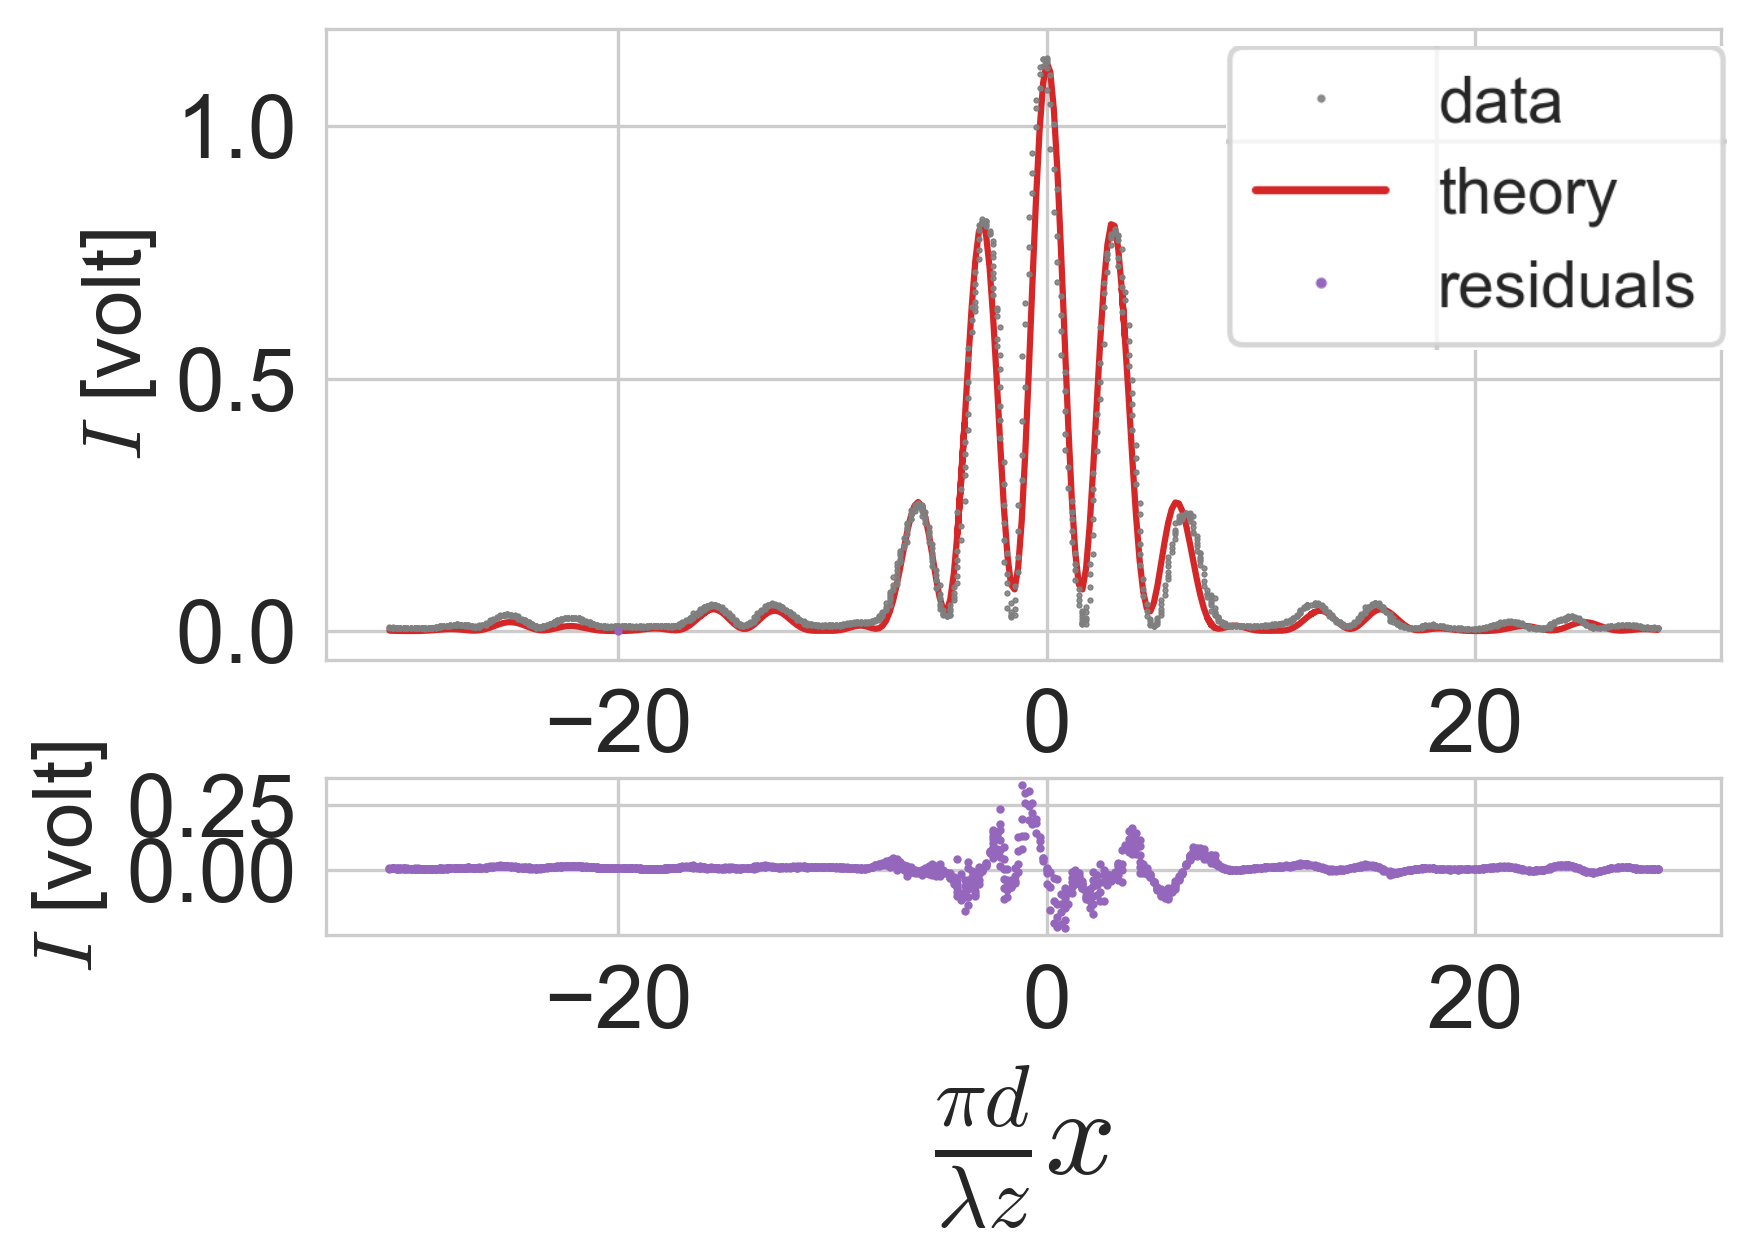
\includegraphics[width=\columnwidth]{figures/0.08w0.25s.png} % first figure itself
        \caption{\\$L=0.25[mm],d=0.08[mm]$}
        \label{fig:double slit interference 0.08w0.25s}
    \end{subfigure}\hfill
    \begin{subfigure}{0.5\columnwidth}
        \centering
        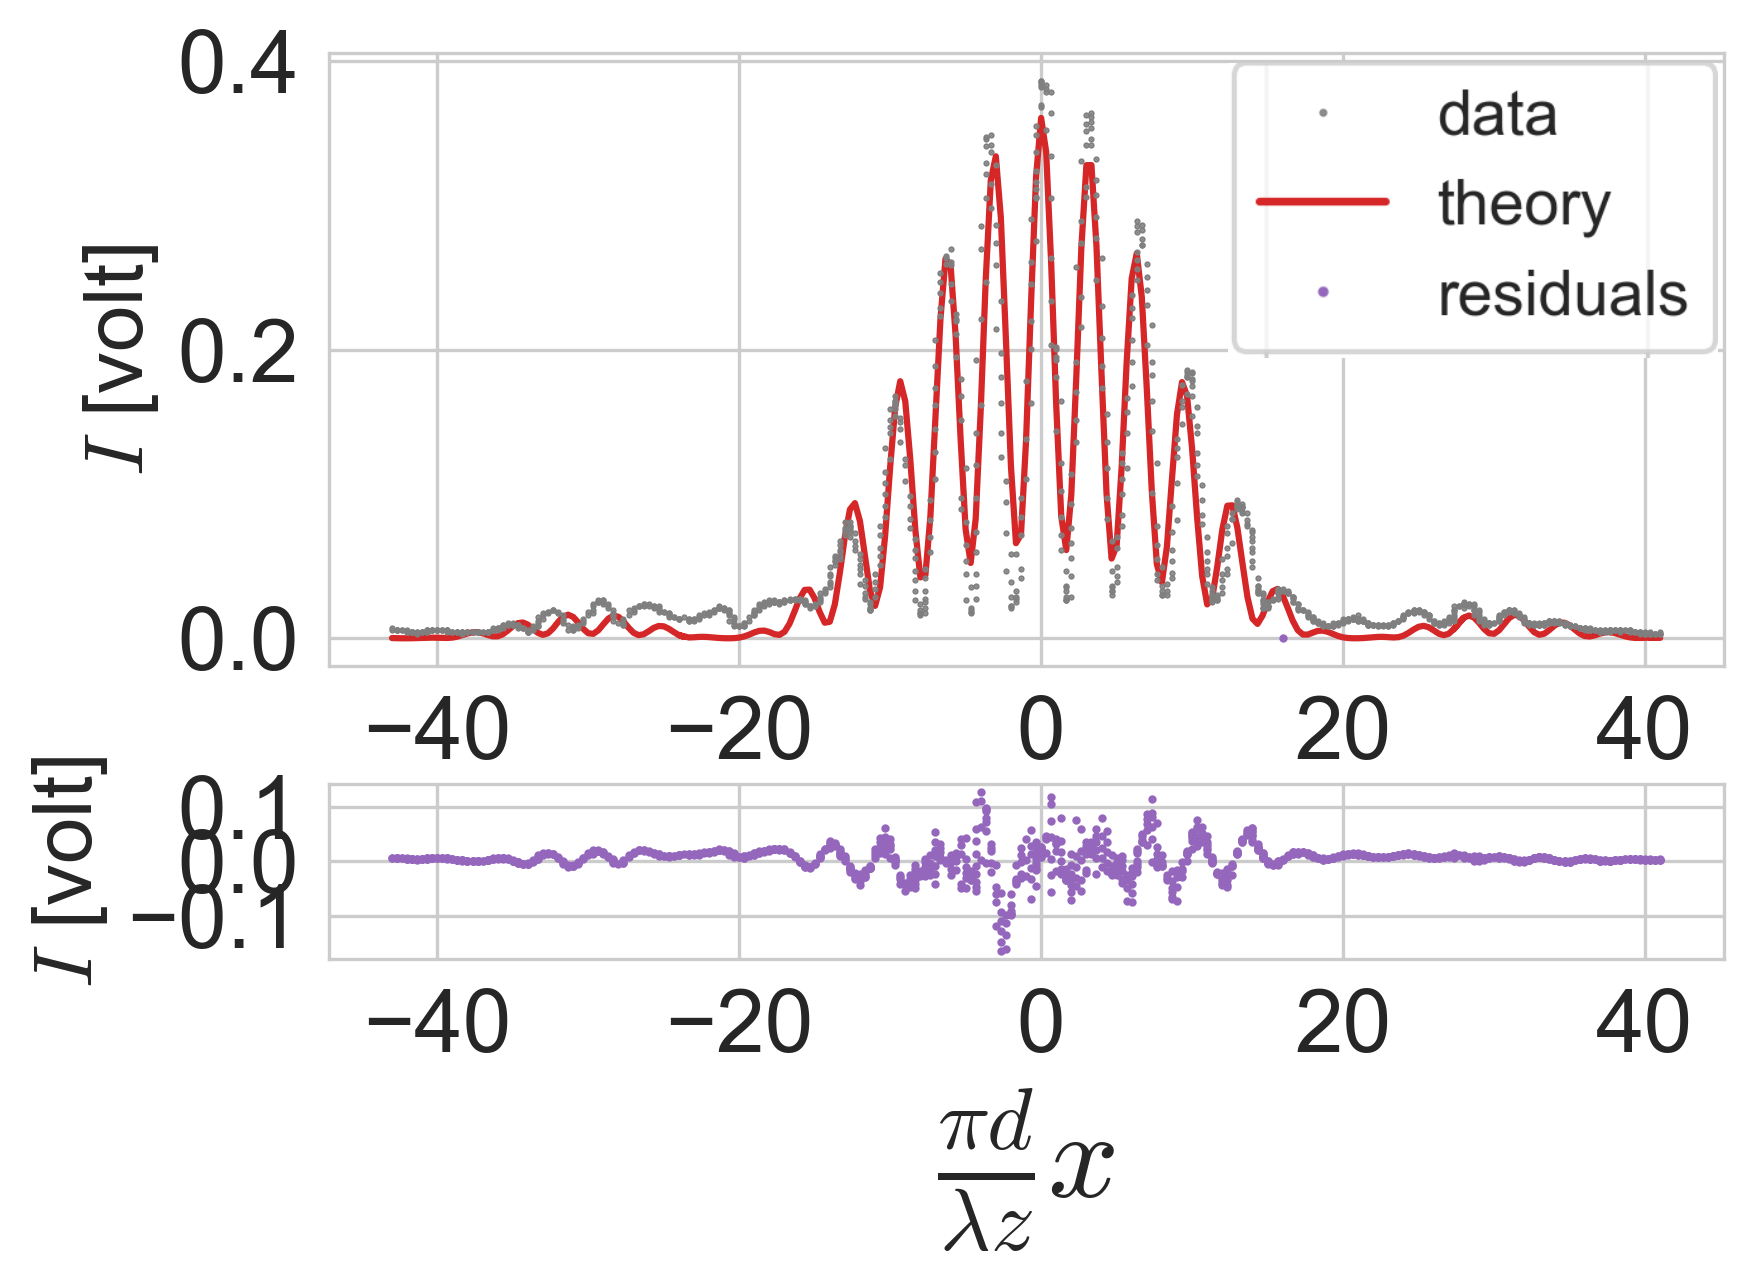
\includegraphics[width=\columnwidth]{figures/0.08w0.5s.png} % second figure itself
        \caption{\\$L=0.5[mm],d=0.08[mm]$}
        \label{fig:double slit interference 0.080.5s}
    \end{subfigure}
    \caption{Diffraction patterns for different slit patterns, for wider slits we get a narrow envelope of main peaks and for greater spacing we see denser peaks.}
    \label{other doubles}
\end{figure}